% !TeX root = ../main.tex

\chapter{信号的描述、分类与基本运算}
\label{chap:signals}

信号描述某个量随自变量的变化。自变量通常是时间，写成 $x(t)$ 或 $x[n]$。信号值可以是实数，也可以是复数。

\section{连续时间信号与离散时间信号}
\label{sec:continuous-and-discrete-signals}

\begin{definition}[连续时间信号]
  \label{def:continuous-time-signal}
  \keyterm{连续时间信号（continuous-time signal）}的自变量连续取值，记
  \[
    x(t),\quad t\in\R.
  \]
\end{definition}

\begin{definition}[离散时间信号]
  \label{def:discrete-time-signal}
  \keyterm{离散时间信号（discrete-time signal）}的自变量只取离散值，默认取整数，记
  \[
    x[n],\quad n\in\Z.
  \]
  也叫\keyterm{序列（sequence）}。方括号提醒我们：$n$ 是离散下标。
\end{definition}

“连续时间”指\red{自变量连续}，不是函数连续。阶跃在跳变点断开，仍是连续时间信号。

“离散时间”也不要求幅值离散，$x[n]$ 仍可以取任意实数或复数。\blue{采样把时间变离散，量化把幅值变离散}，两者分别处理不同方面；量化之后才称为数字信号。

\section{自变量变换与信号运算}
\label{sec:independent-variable-transformations}

设原信号为 $x(t)$，变换后为
\[
  y(t)=x\bigl(g(t)\bigr).
\]
在 $t$ 时刻观察 $y$，实际读取的是原信号在 $g(t)$ 处的值。

作图时只需\hl{跟踪特征点}：端点、峰值、跳变点被移到哪里，图像就画到哪里。括号内的正负号容易看反，不确定时可代入一个点核对。

\subsection{时移}

连续时间时移写成
\begin{equation}
  y(t)=x(t-t_0).
  \label{eq:continuous-time-shift}
\end{equation}
$t_0>0$ 时，原来在 $t=t_1$ 的点移到 $t_1+t_0$，所以图像\red{向右移动} $t_0$，叫\keyterm{延迟（delay）}。$x(t+t_0)$ 则\red{向左移动} $t_0$，叫\keyterm{超前（advance）}。

口诀是\hl{左加右减}，但仅适用于 $x(t-t_0)$ 这种标准形式。括号内带系数时，应先提取系数，或直接解方程。

离散时间规则相同：
\[
  y[n]=x[n-n_0],\qquad n_0\in\Z.
\]
下标必须为整数，因此离散序列\blue{只作整数平移}。

\begin{pitfall}[括号里是减号，图却往右]
  把内部自变量等于原特征点：$t-t_0=t_1$，得 $t=t_1+t_0$。直接解这个方程，比死记口诀可靠。
\end{pitfall}

\subsection{尺度变换与时间反转}

\keyterm{尺度变换}写成
\begin{equation}
  y(t)=x(at),\qquad a\ne0.
  \label{eq:continuous-time-scaling}
\end{equation}
原特征点 $t_1$ 变到 $t_1/a$，所以
\begin{itemize}
  \item $|a|>1$：图像沿时间轴\red{压缩}；
  \item $0<|a|<1$：图像沿时间轴\red{拉伸}；
  \item $a<0$：再\red{关于纵轴翻转}。$x(-t)$ 叫\keyterm{时间反转}。
\end{itemize}
伸缩由\red{系数的绝对值}决定，负号只负责翻转。

尺度变换只改变时间轴，不改变纵坐标。$Ax(t)$ 改变的是幅值，不属于自变量变换。

\begin{pitfall}[离散序列不能照搬伸缩]
  $x[2n]$ 只留下偶数下标；$x[n/2]$ 在奇数 $n$ 处根本没有整数下标。离散尺度变换\blue{须先规定插值或补零}，不能直接套用连续时间的伸缩规则。
\end{pitfall}

\subsection{一般仿射变换}

对
\begin{equation}
  y(t)=x(at+b)
  =x\!\left(a\left(t+\frac{b}{a}\right)\right),
  \qquad a\ne0,
  \label{eq:affine-time-transformation}
\end{equation}
按以下四步：
\begin{enumerate}
  \item \hl{化成标准形式} $x\bigl(a(t-t_0)\bigr)$；
  \item 看 $a$ 的负号，决定要不要翻转；
  \item $|a|>1$ 压缩，$|a|<1$ 拉伸；
  \item 最后平移，口诀\hl{左加右减}。
\end{enumerate}
每一步都\hl{记录端点、峰值和跳变点}，幅度保持不变。完整作图见\cref{ex:signals-affine-triangle}。

作图后可逐点核对。原信号在 $t=\tau$ 处的点，新位置满足
\begin{equation}
  at+b=\tau,
  \qquad
  t=\frac{\tau-b}{a}.
  \label{eq:feature-point-mapping}
\end{equation}
代入几个特征点即可检查位置是否正确。

\begin{example}[画出复合变换的关键位置]
  设 $y(t)=x(-2t+4)=x\bigl(-2(t-2)\bigr)$。先翻转：$\tau\to-\tau$；再压缩：$-\tau\to-\tau/2$；最后右移 $2$：$-\tau/2\to2-\tau/2$。代回核对：
  \[
    -2t+4=\tau,
    \qquad
    t=2-\frac{\tau}{2}.
  \]
  原点 $\tau=0$ 到 $t=2$；原来相距 $2$ 的两点现在只相距 $1$，左右顺序也颠倒。
\end{example}

这套规则的来源：$g(t)$ 增长越快，图像被压得越窄；$g(t)$ 随 $t$ 减小，则从后向前读取，图像反转。\red{改变的是读取原信号的速度和方向}。

\cref{fig:time-transformations}把时移、压缩、反转放在一起比较，峰值和端点的位置与上面的特征点映射一致。

\begin{figure}[htbp]
  \centering
  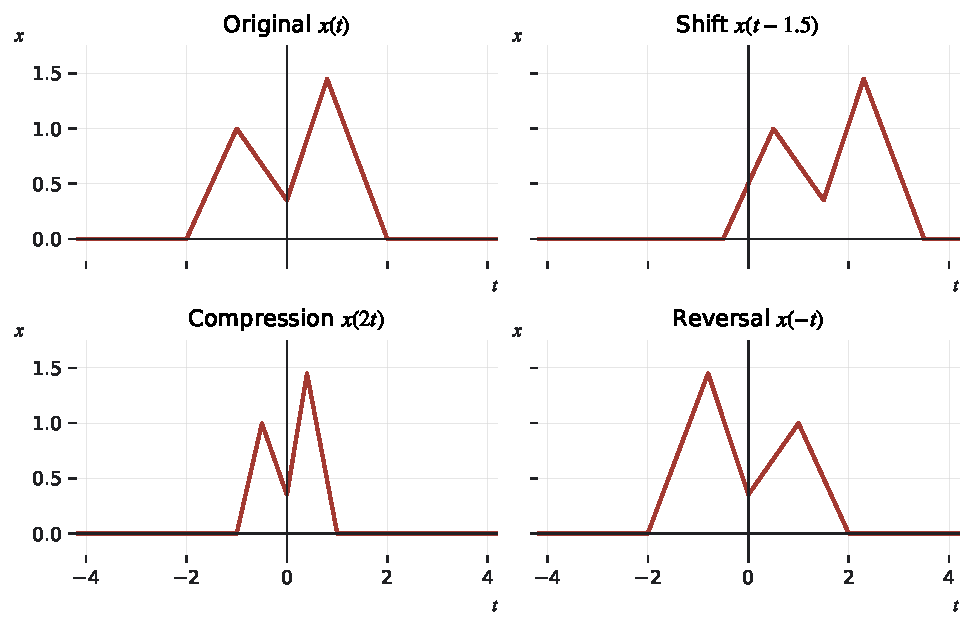
\includegraphics[width=0.88\textwidth]{02-signals/time-transformations.pdf}
  \caption{同一连续时间信号经过时移、压缩和反转后的图像。看峰值和端点的位置，比看公式里的正负号直观。}
  \label{fig:time-transformations}
\end{figure}

\section{周期性、对称性、能量与功率}
\label{sec:signal-properties}

\subsection{周期信号}

\begin{definition}[连续时间周期信号]
  \label{def:continuous-time-periodic-signal}
  若存在 $T>0$，使对任意 $t\in\R$ 都有
  \begin{equation}
    x(t+T)=x(t),
    \label{eq:continuous-time-periodicity}
  \end{equation}
  则 $x(t)$ 是周期信号，$T$ 是它的一个周期。所有正周期中最小的那个叫\keyterm{基波周期（fundamental period）}，记 $T_0$。
\end{definition}

\begin{definition}[离散时间周期信号]
  \label{def:discrete-time-periodic-signal}
  若存在正整数 $N$，使对任意 $n\in\Z$ 都有
  \begin{equation}
    x[n+N]=x[n],
    \label{eq:discrete-time-periodicity}
  \end{equation}
  则 $x[n]$ 是周期序列。最小的正整数叫基波周期，记 $N_0$。
\end{definition}

$T$ 是周期，$2T,3T,\ldots$ 也是。常数信号比较特殊：任意正数都是它的周期，所以\red{没有最小正周期}。

\begin{example}[复指数信号的周期性]
  连续时间复指数 $\e^{\iu\omega_0t}$，$\omega_0\ne0$，基本周期
  \[
    T_0=\frac{2\pi}{|\omega_0|}.
  \]
  离散时间复指数 $\e^{\iu\omega_0n}$ 只有在 $\omega_0/(2\pi)$ 为有理数时才是周期序列。原因是\red{离散周期必须是整数}，$N=2\pi m/\omega_0$ 必须取到整数。
\end{example}

两个连续周期信号相加不一定周期，要求\blue{周期之比为有理数}，才能找到公共周期。离散周期都是整数，有限个相加仍然周期，周期取公倍数。

\subsection{奇信号与偶信号}

\begin{definition}[偶信号]
  \label{def:even-signal}
  满足
  \[
    x(-t)=x(t),\qquad t\in\R
  \]
  的信号叫\keyterm{偶信号（even signal）}。离散形式为 $x[-n]=x[n]$。
\end{definition}

\begin{definition}[奇信号]
  \label{def:odd-signal}
  满足
  \[
    x(-t)=-x(t),\qquad t\in\R
  \]
  的信号叫\keyterm{奇信号（odd signal）}。离散形式为 $x[-n]=-x[n]$。奇信号在原点的值只能是零。
\end{definition}

偶信号关于纵轴对称，奇信号关于原点反对称。这里只翻转时间，\red{信号值不取共轭}，复信号也一样。

\begin{theorem}[奇偶分解]
  任何信号都能\red{唯一拆成一个偶分量加一个奇分量}：
  \begin{align}
    x(t)&=x_{\mathrm e}(t)+x_{\mathrm o}(t),
    \label{eq:even-odd-decomposition}\\
    x_{\mathrm e}(t)&=\frac{x(t)+x(-t)}{2},
    &x_{\mathrm o}(t)&=\frac{x(t)-x(-t)}{2}.
    \label{eq:even-odd-components}
  \end{align}
  离散情形把 $t$ 换成 $n$。
\end{theorem}

\begin{example}[分解多项式信号]
  对 $x(t)=2+t+t^2$，
  \[
    x_{\mathrm e}(t)=2+t^2,
    \qquad
    x_{\mathrm o}(t)=t.
  \]
  相加即还原原信号。偶分量关于纵轴对称，奇分量关于原点反对称，可直接验算。
\end{example}

\cref{fig:even-odd-decomposition}画出了这两部分。

\begin{figure}[htbp]
  \centering
  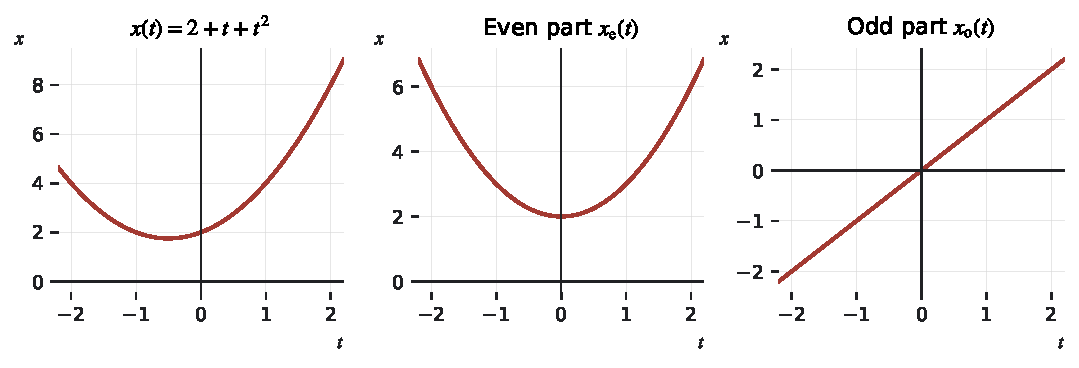
\includegraphics[width=0.92\textwidth]{02-signals/even-odd-decomposition.pdf}
  \caption{$x(t)=2+t+t^2$ 及其偶分量、奇分量。}
  \label{fig:even-odd-decomposition}
\end{figure}

注意，奇偶性\red{相对原点}判断。图像关于 $t=t_0$ 对称，不等于偶信号；先确认对称中心是否为原点。

\subsection{能量信号与功率信号}

把 $x(t)$ 看成 1$\Omega$ 电阻上的电压（或电流），瞬时功率是 $|x(t)|^2$，积分即为能量。连续和离散的定义合写为
\begin{equation}
  E_x=
  \begin{cases}
    \displaystyle\int_{-\infty}^{\infty}|x(t)|^2\dd t,
      &\text{连续时间},\\[0.8em]
    \displaystyle\sum_{n=-\infty}^{\infty}|x[n]|^2,
      &\text{离散时间}.
  \end{cases}
  \label{eq:signal-energy}
\end{equation}
平均功率看长期平均，先在有限区间上取平均，再让区间扩大：
\begin{equation}
  P_x=
  \begin{cases}
    \displaystyle\lim_{T\to\infty}\frac{1}{2T}
      \int_{-T}^{T}|x(t)|^2\dd t,
      &\text{连续时间},\\[1em]
    \displaystyle\lim_{N\to\infty}\frac{1}{2N+1}
      \sum_{n=-N}^{N}|x[n]|^2,
      &\text{离散时间},
  \end{cases}
  \label{eq:average-signal-power}
\end{equation}
\blue{前提是积分、求和与极限都存在}。

\begin{definition}[能量信号与功率信号]
  \label{def:energy-and-power-signals}
  $0<E_x<\infty$ 的叫\keyterm{能量信号（energy signal）}，此时 $P_x=0$。$0<P_x<\infty$ 的叫\keyterm{功率信号（power signal）}，此时 $E_x=\infty$。
\end{definition}

按严格不等式，零信号不属于两者中的任何一类。\blue{考试中遇到零信号，照定义写“既不是能量信号也不是功率信号”}。

周期信号的总能量通常发散，平均功率有限。算功率时取任意一个完整周期即可：
\begin{align}
  P_x&=\frac{1}{T_0}\int_{t_0}^{t_0+T_0}|x(t)|^2\dd t,
  &&\text{连续时间},
  \label{eq:periodic-ct-power}\\
  P_x&=\frac{1}{N_0}\sum_{n=n_0}^{n_0+N_0-1}|x[n]|^2,
  &&\text{离散时间}.
  \label{eq:periodic-dt-power}
\end{align}
起点 $t_0$、$n_0$ 可任取，一个周期内的累积量不变。

\begin{example}[有限时宽脉冲的能量]
  设 $A\ne0$、$T_1>0$，
  \[
    x(t)=
    \begin{cases}
      A,&|t|\leq T_1/2,\\
      0,&\text{其他}.
    \end{cases}
  \]
  则
  \[
    E_x=\int_{-T_1/2}^{T_1/2}|A|^2\dd t=|A|^2T_1,
    \qquad P_x=0.
  \]
  所以它是\red{能量信号}。
\end{example}

\begin{example}[正弦信号的平均功率]
  对 $x(t)=A\cos(\omega_0t+\varphi)$，$A>0$、$\omega_0\ne0$，在一个周期内算得
  \[
    P_x=\frac{A^2}{2}.
  \]
  与初相位无关。信号一直持续，总能量发散，所以\red{是功率信号}。
\end{example}

能量信号与功率信号\red{不是一对互补分类}。$x(t)=t$ 的能量和平均功率都发散，两者都不属于。“不是能量信号”不代表它是功率信号，应回到定义计算。

\section{基本信号与信号分解}
\label{sec:elementary-signals}

\subsection{连续时间单位阶跃信号}

\begin{definition}[单位阶跃信号]
  \label{def:ct-unit-step}
  \keyterm{连续时间单位阶跃信号（unit step signal）}定义为
  \begin{equation}
    \stepfun(t)=
    \begin{cases}
      0,&t<0,\\
      \dfrac{1}{2},&t=0,\\
      1,&t>0.
    \end{cases}
    \label{eq:ct-unit-step}
  \end{equation}
\end{definition}

$t=0$ 这一点，有的书写 $0$，有的写 $1$，有的写 $1/2$；\blue{单点不影响积分}。本书取 $1/2$，与后面频域的对称处理一致。

$\stepfun(t-t_0)$ 在 $t=t_0$ 跳变，之前为零、之后为一，用于表示\red{信号从某时刻开始}。$\stepfun(t_0-t)$ 则在这一刻关闭。

两个移位阶跃相减，可以截出一段：
\begin{equation}
  x(t)=A\bigl[\stepfun(t-t_1)-\stepfun(t-t_2)\bigr],
  \qquad t_1<t_2,
  \label{eq:rectangular-pulse-with-steps}
\end{equation}
在 $(t_1,t_2)$ 内等于 $A$，外面为零。\blue{端点的值由阶跃的零点约定决定}。

\begin{example}[用阶跃信号表示有限时宽脉冲]
  从 $t=-2$ 开始、到 $t=3$ 结束、幅值为 $4$ 的脉冲写成
  \[
    x(t)=4\bigl[\stepfun(t+2)-\stepfun(t-3)\bigr].
  \]
  第一项在 $-2$ 处开启，第二项在 $3$ 处关闭。
\end{example}

判断阶跃的跳变位置，\hl{令括号里的自变量为零}。$\stepfun(2t-4)$ 在 $t=2$ 跳变；判断方向时，再看跳变点两侧的正负。

\subsection{连续时间单位冲激信号}

\begin{definition}[单位冲激信号]
  \label{def:ct-unit-impulse}
  \keyterm{连续时间单位冲激信号（unit impulse signal）}，也叫狄拉克冲激（Dirac delta），记 $\impulse(t)$。它在 $t\ne0$ 处为零，面积为一：
  \begin{equation}
    \int_{-\infty}^{\infty}\impulse(t)\dd t=1.
    \label{eq:unit-area-impulse}
  \end{equation}
  $\impulse(t)$ 是\red{广义函数}：$t=0$ 处没有普通函数值，只在与普通函数积分时起作用。
\end{definition}

移位冲激 $\impulse(t-t_0)$ 集中在 $t=t_0$。$x(t)$ 在 $t_0$ 附近连续时，
\begin{equation}
  \int_{-\infty}^{\infty}
    x(t)\impulse(t-t_0)\dd t=x(t_0).
  \label{eq:ct-impulse-sifting}
\end{equation}
冲激只取出 $x(t_0)$，其余位置不参与积分。

绘制冲激时，\red{箭头高度不是函数值}，旁边的数字表示面积（权重）。

\begin{definition}[冲激的常用性质]
  若 $x(t)$ 在 $t_0$ 附近连续，$a\ne0$，则
  \begin{align}
    \impulse(-t)&=\impulse(t),
    \label{eq:impulse-even}\\
    \impulse(at)&=\frac{1}{|a|}\impulse(t),
    \label{eq:impulse-scaling}\\
    x(t)\impulse(t-t_0)&=x(t_0)\impulse(t-t_0).
    \label{eq:impulse-multiplication}
  \end{align}
  因此
  \begin{equation}
    \impulse(at-b)
    =\frac{1}{|a|}\impulse\!\left(t-\frac{b}{a}\right).
    \label{eq:shifted-scaled-impulse}
  \end{equation}
\end{definition}

\begin{example}[带尺度和位移的冲激]
  化简 $\impulse(3t-6)$：
  \[
    \impulse(3t-6)
    =\frac{1}{3}\impulse(t-2).
  \]
  它位于 $t=2$，权重 $1/3$，总面积为 $1/3$。
\end{example}

缩放时出现 $1/|a|$，因为时间轴压缩后需要补偿面积。\red{绝对值不能丢}；$a<0$ 只把时间反转，不改变面积的符号。

\cref{fig:continuous-step-impulse}是阶跃和冲激的常用画法。

\begin{figure}[htbp]
  \centering
  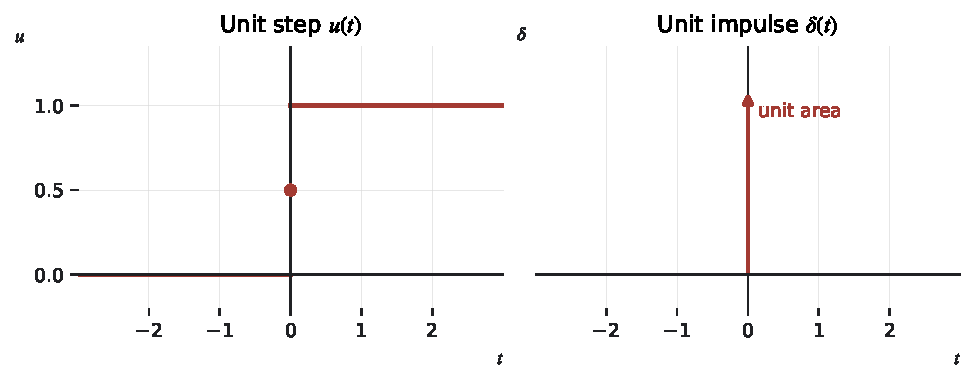
\includegraphics[width=0.82\textwidth]{02-signals/continuous-step-impulse.pdf}
  \caption{连续时间单位阶跃与单位冲激。冲激旁的数字表示面积。}
  \label{fig:continuous-step-impulse}
\end{figure}

阶跃与冲激互为微积分关系：
\begin{align}
  \frac{\dd}{\dd t}\stepfun(t)&=\impulse(t),
  \label{eq:step-derivative-impulse}\\
  \stepfun(t)&=\int_{-\infty}^{t}\impulse(\tau)\dd\tau.
  \label{eq:impulse-integral-step}
\end{align}
第一式在广义函数意义下成立。普通函数在一个瞬间完成跳变，导数无法描述，冲激恰好记录这次跳变的位置和大小。

更一般地，信号在 $t=t_k$ 跳了 $A_k$，广义导数里就多一项 $A_k\impulse(t-t_k)$。\red{向上跳对应正冲激，向下跳对应负冲激}。

\begin{pitfall}[把冲激当成“函数值为无穷大”]
  $\impulse(0)=\infty$ 仅用于直观理解，不能用于计算。实际计算时\hl{使用抽样性质或尺度性质}，看位置、权重和面积。
\end{pitfall}

\subsection{单位阶跃序列与单位冲激序列}

\begin{definition}[单位阶跃序列]
  \label{def:dt-unit-step}
  \keyterm{离散时间单位阶跃序列}定义为
  \begin{equation}
    \stepfun[n]=
    \begin{cases}
      1,&n\geq0,\\
      0,&n<0.
    \end{cases}
    \label{eq:dt-unit-step}
  \end{equation}
\end{definition}

\begin{definition}[单位冲激序列]
  \label{def:dt-unit-impulse}
  \keyterm{离散时间单位冲激序列（unit impulse sequence）}，也叫单位样值序列或 Kronecker delta：
  \begin{equation}
    \impulse[n]=
    \begin{cases}
      1,&n=0,\\
      0,&n\ne0.
    \end{cases}
    \label{eq:dt-unit-impulse}
  \end{equation}
\end{definition}

$\delta[n]$ 是\red{普通序列}，$n=0$ 时就是 $1$。应与 $\delta(t)$ 区分：连续冲激的“值”不是 $1$，离散冲激的值就是 $1$。

\cref{fig:discrete-step-impulse}画出了这两个序列。

\begin{figure}[htbp]
  \centering
  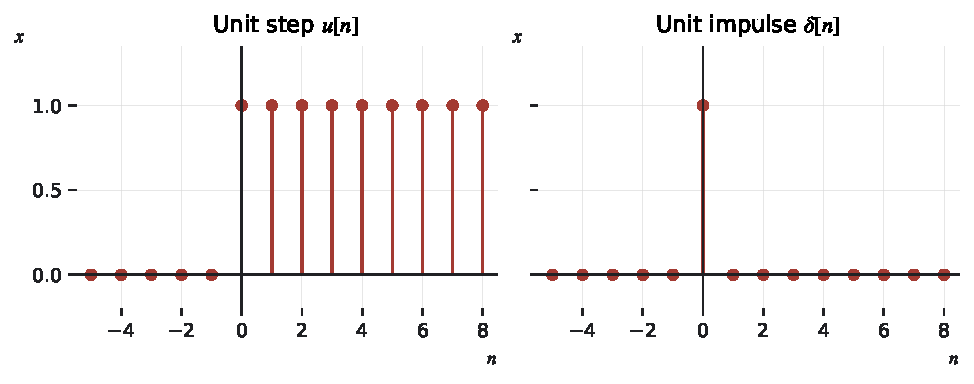
\includegraphics[width=0.82\textwidth]{02-signals/discrete-step-impulse.pdf}
  \caption{离散时间单位阶跃序列与单位冲激序列。每个圆点是一个实际样值。}
  \label{fig:discrete-step-impulse}
\end{figure}

移位冲激只在 $n=n_0$ 处取 $1$，所以
\begin{equation}
  \sum_{k=-\infty}^{\infty}
    x[k]\impulse[k-n_0]=x[n_0].
  \label{eq:dt-impulse-sifting}
\end{equation}

阶跃与冲激通过差分、求和联系：
\begin{align}
  \impulse[n]&=\stepfun[n]-\stepfun[n-1],
  \label{eq:dt-step-difference-impulse}\\
  \stepfun[n]&=\sum_{k=-\infty}^{n}\impulse[k].
  \label{eq:dt-impulse-sum-step}
\end{align}
连续时间用微分寻找跳变；离散时间没有两点之间的值，\red{对应操作改为差分}。

\begin{example}[离散矩形脉冲]
  从 $n=0$ 开始、长度为 $N$ 的矩形脉冲：
  \begin{equation}
    x[n]=\stepfun[n]-\stepfun[n-N],
    \qquad N\in\Z_{>0}.
    \label{eq:dt-rectangular-pulse}
  \end{equation}
  它在 $n=0,1,\ldots,N-1$ 处为 $1$，共 $N$ 个非零样值。最右边是 $N-1$，不是 $N$。
\end{example}

\begin{pitfall}[把连续冲激的尺度规则搬到离散]
  $\impulse[an]=\impulse[n]$（$a$ 为非零整数），\red{没有} $1/|a|$。离散下标只能取整数，$\impulse[an]$ 只是选取了另一些下标，不会产生面积因子。
\end{pitfall}

\subsection{用单位冲激分解信号}

冲激能取出某一时刻的值，将所有时刻的贡献叠加，即还原原信号：
\begin{equation}
  x(t)=\int_{-\infty}^{\infty}
    x(\tau)\impulse(t-\tau)\dd\tau,
  \label{eq:ct-impulse-decomposition}
\end{equation}
\begin{equation}
  x[n]=\sum_{k=-\infty}^{\infty}
    x[k]\impulse[n-k].
  \label{eq:dt-impulse-decomposition}
\end{equation}

以离散式为例：$\impulse[n-k]$ 是位于 $n=k$ 的单位冲激，乘上 $x[k]$ 后高度变成该处的样值。对所有 $k$ 求和，就是把序列逐点重建。连续式表达同一关系，只是求和换成积分。

\begin{example}[用冲激表示有限长序列]
  若 $x[0]=2$、$x[1]=-1$、$x[2]=3$，其余为零，则
  \[
    x[n]=2\impulse[n]-\impulse[n-1]+3\impulse[n-2].
  \]
  每个移位冲激对应一个下标，\red{前面的系数即该处的信号值}。
\end{example}

这一步是卷积的起点：一般信号拆成移位冲激的加权和，LTI 系统只要知道单位冲激响应，就能靠线性和时不变性求出任意输入的响应。后文的\red{冲激响应与卷积}由此得到。

\subsection{抽样函数}
\label{subsec:sampling-function}

\begin{definition}[抽样函数]
  \label{def:sampling-function}
  \keyterm{抽样函数（sampling function）}定义为
  \begin{equation}
    \Sa(t)=
    \begin{cases}
      \dfrac{\sin t}{t},&t\ne0,\\[0.6em]
      1,&t=0.
    \end{cases}
    \label{eq:sampling-function}
  \end{equation}
\end{definition}

原点处直接代入会得到 $0/0$，取极限 $\lim_{t\to0}\sin t/t=1$，所以\red{峰值是 $1$}。

零点在 $t=k\pi$（$k$ 为非零整数）。离原点越远，振荡仍存在，但包络按 $1/|t|$ 衰减。$\Sa(t)$ \red{是偶信号，但不是周期信号}。

\begin{figure}[htbp]
  \centering
  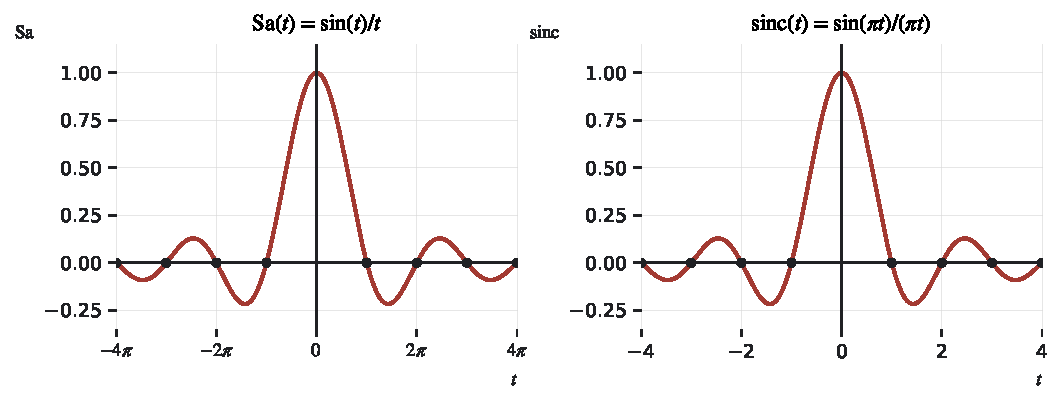
\includegraphics[width=0.88\textwidth]{02-signals/sampling-functions.pdf}
  \caption{非归一化抽样函数 $\Sa(t)$ 与归一化抽样函数 $\sinc(t)$。黑点标出非零零点，两种定义横轴差一个 $\pi$。}
  \label{fig:sampling-functions}
\end{figure}

教材更常用\keyterm{归一化抽样函数}
\begin{equation}
  \sinc(t)=
  \begin{cases}
    \dfrac{\sin(\pi t)}{\pi t},&t\ne0,\\[0.6em]
    1,&t=0,
  \end{cases}
  \qquad
  \sinc(t)=\Sa(\pi t).
  \label{eq:normalized-sinc}
\end{equation}
$\sinc(t)$ 的零点是整数，$\Sa(t)$ 的零点是 $k\pi$。看到 sinc，\blue{先确认定义中是否包含 $\pi$}。

\noindent\textbf{常用性质}
\begin{align}
  \Sa(-t)&=\Sa(t),
  \label{eq:sampling-function-even}\\
  \lim_{|t|\to\infty}\Sa(t)&=0,
  \label{eq:sampling-function-decay}\\
  \int_{-\infty}^{\infty}\Sa(t)\dd t&=\pi,
  \label{eq:sampling-function-area}\\
  \int_{-\infty}^{\infty}|\Sa(t)|^2\dd t&=\pi.
  \label{eq:sampling-function-energy}
\end{align}
对应地，
\[
  \int_{-\infty}^{\infty}\sinc(t)\dd t=1,
  \qquad
  \int_{-\infty}^{\infty}|\sinc(t)|^2\dd t=1.
\]
第一个积分条件收敛；第二个积分说明\red{抽样函数是能量信号}。

\noindent\textbf{面积怎么算}
引入参数 $a>0$：
\[
  I(a)=\int_0^\infty\e^{-at}\frac{\sin t}{t}\dd t.
\]
$\e^{-at}$ 保证积分绝对收敛。对 $a$ 求导，再用欧拉公式把正弦拆开：
\begin{align*}
  I'(a)
  &=-\int_0^\infty\e^{-at}\sin t\dd t\\
  &=-\frac1{2\iu}\int_0^\infty
      \left[\e^{-(a-\iu)t}-\e^{-(a+\iu)t}\right]\dd t\\
  &=-\frac1{2\iu}\left(\frac1{a-\iu}-\frac1{a+\iu}\right)
   =-\frac1{a^2+1}.
\end{align*}
于是 $I(a)=-\arctan a+C$。又 $|\sin t/t|\le1$，所以 $|I(a)|\le1/a$，$a\to\infty$ 时 $I(a)\to0$，定出
\[
  C=\frac{\pi}{2},\qquad I(a)=\frac{\pi}{2}-\arctan a.
\]
令 $a\to0^+$，得 $\int_0^\infty\sin t/t\dd t=\pi/2$。由偶性，
\[
  \int_{-\infty}^{\infty}\frac{\sin t}{t}\dd t
    =2\times\frac{\pi}{2}=\pi.
\]
平方积分见\cref{eg:ctft-sinc-energy}。

\hl{参数积分：引入衰减因子，求导，再令参数趋于零}。这是计算此类积分的常用方法。

尺度和平移决定主瓣的位置和宽度：
\begin{equation}
  x(t)=A\Sa\bigl(B(t-t_0)\bigr),
  \label{eq:scaled-shifted-sampling-function}
\end{equation}
峰值在 $t=t_0$，取 $A$；零点在
\[
  t=t_0+\frac{k\pi}{B},
  \qquad k\in\Z\setminus\{0\}.
\]
$B$ 越大，\red{零点越密，主瓣越窄}。能量为
\begin{equation}
  E_x=\frac{|A|^2\pi}{B}.
  \label{eq:scaled-sampling-function-energy}
\end{equation}

\begin{example}[读取抽样函数的峰值、零点与能量]
  设 $x(t)=3\Sa\bigl(2(t-1)\bigr)$。峰值在 $t=1$，等于 $3$；零点在
  \[
    t=1+\frac{k\pi}{2},
    \qquad k\in\Z\setminus\{0\}.
  \]
  能量 $E_x=9\pi/2$。
\end{example}

改变 $B$ 时，主瓣、旁瓣、零点按同一比例伸缩。到傅里叶变换中，就表现为\red{“时域越窄，频域越宽”}；理想低通和带限重建都会用到抽样函数。

“抽样函数”是一个确定的连续时间函数；“对信号抽样”是另一种操作。名称相近，含义不同。采样和混叠见\cref{chap:sampling}。
